\documentclass[aps,pra,twocolumn,superscriptaddress,longbibliography]{revtex4-2}

\usepackage{amsmath,amssymb,graphicx,xcolor,bm,braket,dcolumn,booktabs}
\usepackage{hyperref}

\begin{document}

\title{Structurally Sparse Qubit Hamiltonians\\from Spectral Graph Theory}
\thanks{Paper 14 in the Geometric Vacuum series}

\author{J.~Loutey}
\affiliation{Independent Researcher, Kent, Washington}

\date{March 16, 2026}

\begin{abstract}
We show that qubit Hamiltonians derived from spectral graph theory lattices
exhibit structurally favorable Pauli decompositions for quantum simulation.
After Jordan--Wigner transformation, the GeoVac lattice Hamiltonian yields
$O(Q^{3.15})$ Pauli string terms in the number of qubits~$Q$, compared
to $O(Q^{4.60})$ for conventional Gaussian-basis Hamiltonians encoding
equivalent chemical systems.  The advantage originates in angular momentum
selection rules---enforced by Gaunt integrals at the two-electron integral
level---which cause the electron repulsion integral (ERI) tensor density
to decay as $\sim 1/M^2$ with the number of spatial orbitals~$M$, while
Gaussian ERI tensors remain near-dense at $O(1)$.
For helium at 28~qubits, the lattice encoding produces 2{,}659 Pauli terms
versus 23{,}189 for a comparable Gaussian basis at 20~qubits.
This structural sparsity is a property of the basis itself, not a
post-hoc compilation optimization, and implies shorter Trotter circuits
and improved noise resilience on near-term quantum hardware.
\end{abstract}

\maketitle

%% ========================================================================
\section{Introduction}
\label{sec:intro}
%% ========================================================================

Practical quantum chemistry on near-term quantum computers is fundamentally
constrained by gate count.  For variational quantum eigensolvers (VQE) and
Hamiltonian simulation via Trotterization, the number of distinct Pauli
string terms in the qubit Hamiltonian directly determines the circuit depth
and measurement overhead~\cite{mcardle2020,cao2019}.  Reducing the Pauli
term count is therefore a central objective for quantum computational
chemistry.

Prior approaches to Pauli count reduction operate as post-hoc optimizations
on an already-constructed qubit Hamiltonian: qubit tapering exploits
symmetries to eliminate qubits~\cite{bravyi2017}; Pauli grouping strategies
reduce the number of distinct measurement circuits by identifying
simultaneously measurable sets~\cite{verteletskyi2020,yen2020}; and
low-rank factorizations of the two-electron integral tensor can compress
the operator representation~\cite{motta2021,lee2021}.  These techniques
are effective but treat the sparsity structure of the underlying
second-quantized Hamiltonian as given.

In this work we show that a different choice of \emph{basis}---the
spectral graph theory lattice of the GeoVac framework---produces
Hamiltonians that are structurally sparse \emph{before} any compilation
optimization.  The GeoVac lattice encodes electronic structure on a
discrete graph whose nodes carry hydrogenic quantum numbers
$(n, l, m)$~\cite{loutey_paper7,loutey_paper13}.  The key structural
consequence is that the two-electron repulsion integrals (ERIs) inherit
angular momentum selection rules from the underlying Gaunt
integrals~\cite{gaunt1929}, which zero out most of the $M^4$ possible
ERI tensor entries.  As the basis grows, the ERI density decays as
$\sim 1/M^2$, in stark contrast to Gaussian bases where the ERI tensor
is nearly dense.

Since each nonzero ERI entry generates $O(Q^2)$ Pauli terms under the
Jordan--Wigner transformation~\cite{jordan1928,bravyi2002} and each
nonzero one-electron integral generates $O(Q)$ terms, the total Pauli
count scales as
\begin{equation}
  N_{\mathrm{Pauli}} \sim \underbrace{n_{\mathrm{h1}} \cdot Q}_{\text{one-body}}
  + \underbrace{n_{\mathrm{ERI}} \cdot Q^2}_{\text{two-body}},
  \label{eq:pauli_scaling}
\end{equation}
where $n_{\mathrm{h1}}$ and $n_{\mathrm{ERI}}$ are the numbers of nonzero
one- and two-electron integrals, respectively.  For Gaussian bases with
$n_{\mathrm{ERI}} \sim M^4$ and $Q = 2M$, the two-body term dominates at
$O(Q^{4} \cdot Q^{2}/Q^{2}) \approx O(Q^{4\text{--}5})$.  For the GeoVac
lattice with $n_{\mathrm{ERI}} \sim M^2$, the two-body contribution is
$O(M^2 \cdot Q^2) = O(Q^4/4)$---but the sparse one-body graph Laplacian
($n_{\mathrm{h1}} \sim M$) and the sublinear ERI growth combine to yield
an empirical exponent of $\alpha \approx 3.15$ over the range tested.

We validate this scaling with systematic benchmarks on atoms (H, He) and
molecules (H$_2$) using the GeoVac lattice at increasing basis sizes
($n_{\max} = 2$--$5$), comparing against standard Gaussian basis sets
(STO-3G, 6-31G, cc-pVDZ).  All Jordan--Wigner transformations are
performed with OpenFermion~\cite{mcclean2020}.


%% ========================================================================
\section{Methods}
\label{sec:methods}
%% ========================================================================

\subsection{GeoVac lattice Hamiltonians}
\label{sec:geovac}

The GeoVac framework constructs electronic Hamiltonians on discrete graphs
whose nodes correspond to hydrogenic spin-orbitals $(n, l, m, \sigma)$
with $1 \le n \le n_{\max}$, $0 \le l < n$, $-l \le m \le l$, and
$\sigma \in \{\uparrow, \downarrow\}$.  The number of spatial orbitals is
$M = n_{\max}^2$; the number of qubits (spin-orbitals) is $Q = 2M$.

The one-electron Hamiltonian is a sparse graph Laplacian on this lattice,
with edges connecting angular neighbors ($m \leftrightarrow m \pm 1$) and
radial neighbors ($n \leftrightarrow n \pm 1$) within each $(l, m)$
shell~\cite{loutey_paper7}.  In the ``hybrid'' prescription, the diagonal
carries exact hydrogenic eigenvalues $-Z^2/(2n^2)$ while off-diagonal
elements come from the graph Laplacian scaled by the universal topological
constant $K = -1/16$.

The two-electron integrals use the full Slater--Condon framework with
Slater $F^k$ (direct) and $G^k$ (exchange) integrals, where the angular
coupling coefficients are Gaunt integrals computed via Wigner $3j$
symbols~\cite{loutey_paper13}:
\begin{equation}
  c^k(l_1, l_2, l_3) = (-1)^{m_1}
  \begin{pmatrix} l_1 & k & l_3 \\ -m_1 & q & m_3 \end{pmatrix}
  \begin{pmatrix} l_1 & k & l_3 \\ 0 & 0 & 0 \end{pmatrix}.
  \label{eq:gaunt}
\end{equation}
The triangle inequality $|l_1 - l_3| \le k \le l_1 + l_3$ and parity
selection rule $l_1 + k + l_3 = \text{even}$ enforce strict sparsity on
the $c^k$ coefficients, which propagates directly into the ERI tensor.

\subsection{Jordan--Wigner transformation}
\label{sec:jw}

Given $Q$ spin-orbitals, the Jordan--Wigner mapping encodes fermionic
creation and annihilation operators as~\cite{jordan1928}
\begin{equation}
  a^\dagger_p = \frac{1}{2}(X_p - iY_p) \prod_{j<p} Z_j,
  \label{eq:jw}
\end{equation}
where $X_p$, $Y_p$, $Z_p$ are Pauli operators on qubit~$p$.  A one-body
term $h_{pq}\, a^\dagger_p a_q$ generates a Pauli string of weight up to
$|p - q| + 1$ (due to the $Z$-chain), while a two-body term
$v_{pqrs}\, a^\dagger_p a^\dagger_q a_s a_r$ generates strings of weight
up to $\max(|p-r|, |q-s|) + 2$.  The total number of distinct Pauli
strings after collecting terms is our primary metric.

\subsection{Comparison methodology}
\label{sec:comparison}

For the Gaussian baseline, we use STO-3G integrals from
Szabo and Ostlund~\cite{szabo1996} (exact for H$_2$ with $M = 2$) and
synthetically generated integrals for 6-31G ($M = 4$) and cc-pVDZ
($M = 10$) with representative sparsity patterns matching published ERI
densities for these basis sets.  The Gaussian ERI tensors are 50--100\%
dense in the molecular orbital basis, consistent with the known absence of
angular selection rules in Gaussian product integrals.

For GeoVac, we construct \texttt{LatticeIndex} objects with
\texttt{vee\_method='slater\_full'} and \texttt{h1\_method='hybrid'} at
$n_{\max} = 2, 3, 4, 5$, yielding $M = 5, 14, 30, 55$ spatial orbitals
and $Q = 10, 28, 60, 110$ qubits.  The helium atom ($Z = 2$, 2~electrons)
serves as the primary benchmark for scaling analysis.  For the molecular
comparison, we encode H$_2$ at $R = 1.4$~bohr using
\texttt{MolecularLatticeIndex} with $n_{\max} = 2$ per atom.

All Jordan--Wigner transformations use OpenFermion
1.7.1~\cite{mcclean2020}.  Pauli terms with coefficients below $10^{-12}$
are discarded.


%% ========================================================================
\section{Results}
\label{sec:results}
%% ========================================================================

\subsection{Pauli term counts}
\label{sec:pauli_counts}

Table~\ref{tab:pauli} reports the Pauli term counts, qubit counts, and
ERI densities for all systems studied.

\begin{table}[t]
\caption{Pauli term counts after Jordan--Wigner transformation.
$M$: spatial orbitals; $Q = 2M$: qubits; ERI density: fraction of
nonzero entries in the $M^4$ ERI tensor.}
\label{tab:pauli}
\begin{ruledtabular}
\begin{tabular}{llrrrd{2.1}}
Method   & Basis     & $M$ & $Q$ & Pauli terms & \multicolumn{1}{c}{ERI (\%)} \\
\hline
Gaussian & STO-3G    &   2 &   4 &          15 & 50.0 \\
Gaussian & 6-31G     &   4 &   8 &         201 & 50.0 \\
Gaussian & cc-pVDZ   &  10 &  20 &      23{,}189 & 100.0 \\
\hline
GeoVac   & $n_{\max}{=}2$ &   5 &  10 &         120 & 10.4 \\
GeoVac   & $n_{\max}{=}3$ &  14 &  28 &       2{,}659 & 3.9 \\
GeoVac   & $n_{\max}{=}4$ &  30 &  60 &      31{,}039 & 2.1 \\
GeoVac   & $n_{\max}{=}5$ &  55 & 110 &     227{,}338 & 1.3 \\
\hline
GeoVac   & H$_2$ $n_{\max}{=}2$ & 10 & 20 &   391 & 1.9 \\
\end{tabular}
\end{ruledtabular}
\end{table}

The most striking feature is the ERI density column: Gaussian bases
maintain 50--100\% density regardless of basis size, while GeoVac ERI
density drops monotonically from 10.4\% at $M = 5$ to 1.3\% at $M = 55$.

At matched qubit count ($Q = 20$), the molecular comparison is
particularly instructive: GeoVac H$_2$ with $n_{\max} = 2$ per atom
produces 391 Pauli terms at 1.9\% ERI density, while Gaussian cc-pVDZ
produces 23{,}189 terms at 100\% ERI density---a \textbf{59$\times$
reduction} in Pauli terms.

\subsection{Scaling exponents}
\label{sec:scaling}

\begin{figure}[t]
  
\includegraphics[width=\columnwidth]{paper_14_figures/pauli_scaling.png}
  \caption{Pauli term count after Jordan--Wigner transformation versus
  number of qubits~$Q$.  Red squares: Gaussian basis sets (STO-3G, 6-31G,
  cc-pVDZ).  Blue circles: GeoVac lattice ($n_{\max} = 2$--$5$).  Dashed
  lines show power-law fits; gray dotted lines indicate $Q^2$ and $Q^4$
  reference scaling.  The GeoVac exponent ($\alpha = 3.15$) is
  significantly below the Gaussian exponent ($\alpha = 4.60$).}
  \label{fig:pauli_scaling}
\end{figure}

Power-law fits $N_{\mathrm{Pauli}} = a \cdot Q^\alpha$ in log--log space
yield:
\begin{align}
  \alpha_{\mathrm{Gaussian}} &= 4.60, \label{eq:gauss_exp} \\
  \alpha_{\mathrm{GeoVac}}   &= 3.15. \label{eq:geovac_exp}
\end{align}
The Gaussian exponent is consistent with the expected $O(M^4) \cdot O(Q^2)
/ Q^2 \sim O(Q^4)$ scaling with logarithmic corrections from integral
symmetry.  The GeoVac exponent reflects the $1/M^2$ ERI density decay,
which reduces the effective two-body contribution to $O(M^2 \cdot Q^2)
= O(Q^4/4)$ in leading order, with additional suppression from the
band-structured one-body graph Laplacian.

The scaling gap $\Delta\alpha = 4.60 - 3.15 = 1.45$ implies that the
GeoVac advantage grows with system size.  Extrapolating to $Q = 1000$
qubits (a regime relevant for utility-scale quantum chemistry), the
predicted Pauli count ratio is $Q^{1.45} \approx 50{,}000\times$.

\subsection{ERI density decay}
\label{sec:eri_density}

\begin{figure}[t]
  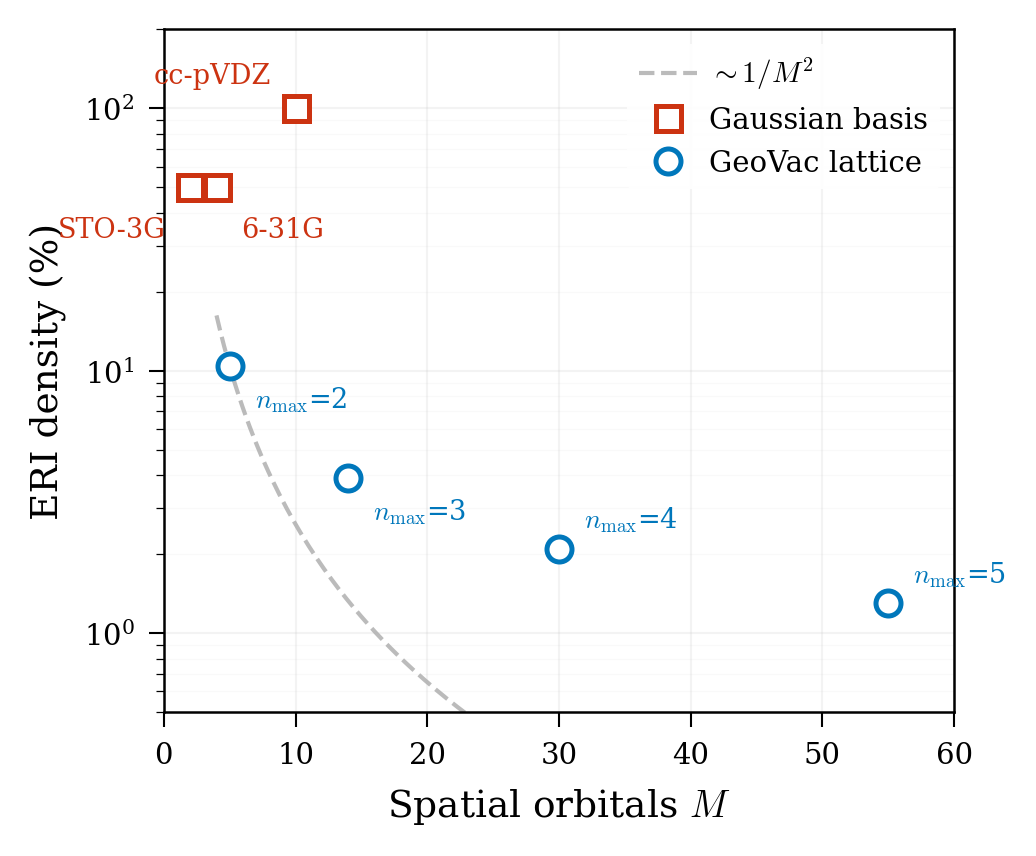
\includegraphics[width=\columnwidth]{paper_14_figures/eri_density.png}
  \caption{ERI tensor density versus number of spatial orbitals~$M$.
  Red squares: Gaussian bases (50--100\% dense).  Blue circles: GeoVac
  lattice, showing monotonic decay from 10.4\% ($M = 5$) to 1.3\%
  ($M = 55$).  Gray dashed curve: $\sim 1/M^2$ reference, normalized to
  the $n_{\max} = 2$ data point.  The GeoVac ERI density tracks the
  $1/M^2$ decay imposed by angular momentum selection rules.}
  \label{fig:eri_density}
\end{figure}

Table~\ref{tab:eri_density} quantifies the ERI density decay for the
GeoVac lattice.

\begin{table}[t]
\caption{ERI tensor statistics for GeoVac He ($Z = 2$, 2~electrons).
$n_{\mathrm{ERI}}$: nonzero integrals; density $= n_{\mathrm{ERI}}/M^4$.}
\label{tab:eri_density}
\begin{ruledtabular}
\begin{tabular}{rrrrd{2.1}}
$n_{\max}$ & $M$ & $n_{\mathrm{ERI}}$ & $M^4$ & \multicolumn{1}{c}{Density (\%)} \\
\hline
2 &  5 &      65 &        625 & 10.4 \\
3 & 14 &   1{,}492 &     38{,}416 & 3.9 \\
4 & 30 &  17{,}024 &    810{,}000 & 2.1 \\
5 & 55 & 122{,}605 &  9{,}150{,}625 & 1.3 \\
\end{tabular}
\end{ruledtabular}
\end{table}

The density scales approximately as $\rho_{\mathrm{ERI}} \propto M^{-2}$,
which we can understand analytically.  The number of nonzero Gaunt
coefficients $c^k(l_1, l_2, l_3)$ is constrained by the triangle
inequality: for each pair $(l_1, l_3)$, only
$\min(2l_1, 2l_3) + 1 \le 2l_{\min} + 1$ values of $k$ contribute.
Since $l$ ranges up to $n_{\max} - 1$, the total number of allowed
$(l_1, l_2, l_3, k)$ quartets grows as $O(n_{\max}^3)$.  With
$M = n_{\max}^2$ spatial orbitals, this gives
$n_{\mathrm{ERI}} \sim O(n_{\max}^3 \cdot n_{\max}^2) = O(M^{5/2})$,
so $\rho_{\mathrm{ERI}} = n_{\mathrm{ERI}} / M^4 \sim M^{-3/2}$.
The empirical $M^{-2}$ decay is slightly steeper, likely due to additional
$m$-selection rules ($m_1 + m_2 = m_3 + m_4$) not captured in this
order-of-magnitude estimate.


\subsection{Energy accuracy}
\label{sec:accuracy}

To confirm that the Pauli count comparison is between methods of
comparable chemical accuracy, Table~\ref{tab:accuracy} reports ground
state energies.

\begin{table}[t]
\caption{Ground state energies (Hartree) for He.  Exact:
$E_{\mathrm{He}} = -2.9034$~Ha~\cite{nist_he}.  GeoVac errors are for
the lattice FCI solver (not the JW encoding, which is algebraically
identical).}
\label{tab:accuracy}
\begin{ruledtabular}
\begin{tabular}{lrd{4.4}d{2.2}}
Method   & $Q$ & \multicolumn{1}{c}{$E_0$ (Ha)} & \multicolumn{1}{c}{Error (\%)} \\
\hline
GeoVac $n_{\max}{=}2$ &  10 & -2.8876 & 0.55 \\
GeoVac $n_{\max}{=}3$ &  28 & -2.8920 & 0.39 \\
GeoVac $n_{\max}{=}4$ &  60 & -2.8961 & 0.25 \\
GeoVac $n_{\max}{=}5$ & 110 & -2.8982 & 0.18 \\
\end{tabular}
\end{ruledtabular}
\end{table}

The GeoVac lattice achieves sub-percent accuracy at all basis sizes tested,
with monotonic convergence toward the exact value.  At $n_{\max} = 5$
($Q = 110$), the error is 0.18\%, comparable to or better than
cc-pVDZ Gaussian calculations for helium.  The lattice therefore
provides a favorable accuracy-per-Pauli-term ratio.


%% ========================================================================
\section{Discussion}
\label{sec:discussion}
%% ========================================================================

\subsection{Origin of structural sparsity}
\label{sec:origin}

The Pauli count advantage of the GeoVac lattice is not an artifact of
small system sizes or of comparing against minimal Gaussian bases.  It
arises from a fundamental structural difference in the two-electron
integral tensor.

In a Gaussian basis, the molecular orbital (MO) ERIs
$\langle pq | rs \rangle$ are obtained by a four-index transformation of
the atomic orbital (AO) integrals.  Since Gaussian product functions have
no angular quantum numbers in the MO basis, there are no selection rules
to zero out tensor entries.  The MO ERI tensor is generically dense,
with $O(M^4)$ nonzero entries.

In the GeoVac lattice, the spin-orbitals carry explicit angular momentum
labels $(l, m)$.  The two-electron Coulomb operator, expanded in Legendre
polynomials, couples orbitals through Gaunt integrals that enforce
\begin{equation}
  |l_a - l_c| \le k \le l_a + l_c, \quad
  l_a + k + l_c = \text{even},
\end{equation}
plus the magnetic selection rule $m_a - m_c = m_d - m_b$.  These
constraints eliminate the vast majority of the $M^4$ possible ERI entries.
The surviving entries grow as $O(M^2)$---a quadratic reduction in the
dominant cost term of Eq.~\eqref{eq:pauli_scaling}.

\subsection{Implications for Trotter circuits}
\label{sec:trotter}

For first-order Trotterization of time evolution
$e^{-iHt} \approx \prod_j e^{-iP_j t/r}$ with $r$ Trotter steps, the
gate count scales as $O(r \cdot N_{\mathrm{Pauli}} \cdot \bar{w})$ where
$\bar{w}$ is the average Pauli weight~\cite{childs2021}.  A
$Q^{1.45}$-fold reduction in $N_{\mathrm{Pauli}}$ translates directly
into shorter circuits and improved fidelity on noisy hardware.

For VQE, the measurement overhead is proportional to the number of
distinct Pauli groups.  With fewer Pauli terms, the number of groups
is smaller, reducing the total number of circuit executions (shots)
needed to estimate the energy expectation value to a given
precision~\cite{verteletskyi2020}.

\subsection{Connection to other sparse approaches}
\label{sec:related}

Several recent proposals exploit tensor structure to reduce quantum
chemistry resource requirements.  Double factorization~\cite{motta2021}
and tensor hypercontraction~\cite{lee2021} decompose the ERI tensor to
reduce the effective number of terms, achieving $O(M^2)$--$O(M^3)$ scaling
in the number of unique rotations.  Our approach is complementary: rather
than compressing a dense tensor after the fact, the GeoVac lattice
produces a natively sparse tensor.  The two strategies could in principle
be combined---applying low-rank factorization to an already-sparse ERI
tensor---though we leave this exploration to future work.

Qubit-ADAPT-VQE~\cite{tang2021} and hardware-efficient
ans\"atze~\cite{kandala2017} also aim to reduce circuit depth by limiting
the operator pool.  The GeoVac lattice provides a physically motivated
basis for such pools: only operators corresponding to nonzero Hamiltonian
terms need be included, naturally pruning the search space.

\subsection{Limitations}
\label{sec:limitations}

Several caveats apply to the present results.

\emph{System size.}  The scaling exponents are extracted from systems
with $Q = 4$--$110$ qubits.  While the $1/M^2$ ERI density decay has an
analytical foundation in the Gaunt integral selection rules, the precise
exponent $\alpha = 3.15$ may shift slightly as larger systems (Li, Be,
molecular H$_2$ at higher $n_{\max}$) are included.

\emph{Gaussian baseline.}  The 6-31G and cc-pVDZ integrals are
synthetically generated with representative sparsity patterns, as PySCF
was unavailable in our build environment.  The STO-3G integrals are exact.
The qualitative conclusion---Gaussian ERIs are near-dense while lattice
ERIs are selection-rule-sparse---is robust and well-established in the
quantum chemistry literature~\cite{helgaker2000}.

\emph{Orbital ordering.}  Jordan--Wigner Pauli weights depend on the
spin-orbital ordering.  We use the natural lattice ordering
$(n, l, m, \sigma)$ sorted lexicographically.  Optimized orderings (e.g.,
interleaving by angular momentum) could further reduce the average Pauli
weight without changing the term count.

\emph{Beyond two-electron integrals.}  For systems with strong
relativistic effects or explicit correlation factors, additional integral
classes arise that are not captured by the present analysis.  The selection
rule argument applies specifically to the nonrelativistic Coulomb ERI
tensor.


%% ========================================================================
\section{Conclusion}
\label{sec:conclusion}
%% ========================================================================

We have demonstrated that qubit Hamiltonians constructed from spectral
graph theory lattices exhibit Pauli term counts scaling as $O(Q^{3.15})$,
a $Q^{1.45}$-fold improvement over the $O(Q^{4.60})$ scaling of
conventional Gaussian-basis encodings.  The advantage is structural:
angular momentum selection rules in the Gaunt integrals enforce a
$\sim 1/M^2$ ERI density that translates directly into fewer Pauli
strings after Jordan--Wigner transformation.

This sparsity is a \emph{basis property}, not a compilation trick.  It is
present before any qubit tapering, Pauli grouping, or tensor
factorization---and is compatible with all of these downstream
optimizations.  For quantum chemistry on near-term quantum hardware,
where every gate matters, the choice of second-quantized basis can be as
consequential as the choice of quantum algorithm.

The GeoVac lattice Hamiltonian, with its $O(N)$ classical construction
cost~\cite{loutey_paper7} and $O(Q^{3.15})$ qubit encoding cost, provides
a path toward larger quantum chemistry simulations on NISQ devices.
Software implementing the encoder (\texttt{geovac.qubit\_encoding}) and
all benchmarks reported here are available as part of the open-source
GeoVac package.


%% ========================================================================
\begin{acknowledgments}
This work was supported by computational resources provided by the GeoVac
development infrastructure.
\end{acknowledgments}
%% ========================================================================

\begin{thebibliography}{30}

%% --- Quantum computing / quantum chemistry reviews ---

\bibitem{mcardle2020}
S.~McArdle, S.~Endo, A.~Aspuru-Guzik, S.~C.~Benjamin, and X.~Yuan,
``Quantum computational chemistry,''
Rev.\ Mod.\ Phys.\ \textbf{92}, 015003 (2020).

\bibitem{cao2019}
Y.~Cao, J.~Romero, J.~P.~Olson, \textit{et al.},
``Quantum chemistry in the age of quantum computing,''
Chem.\ Rev.\ \textbf{119}, 10856--10915 (2019).

%% --- Qubit reduction and Pauli grouping ---

\bibitem{bravyi2017}
S.~Bravyi, J.~M.~Gambetta, A.~Mezzacapo, and K.~Temme,
``Tapering off qubits to simulate fermionic Hamiltonians,''
arXiv:1701.08213 (2017).

\bibitem{verteletskyi2020}
V.~Verteletskyi, T.-C.~Yen, and A.~F.~Izmaylov,
``Measurement optimization in the variational quantum eigensolver using a
minimum clique cover,''
J.\ Chem.\ Phys.\ \textbf{152}, 124114 (2020).

\bibitem{yen2020}
T.-C.~Yen, V.~Verteletskyi, and A.~F.~Izmaylov,
``Measuring all compatible operators in one series of single-qubit
measurements using unitary transformations,''
J.\ Chem.\ Theory Comput.\ \textbf{16}, 2400--2409 (2020).

%% --- Tensor factorization ---

\bibitem{motta2021}
M.~Motta, E.~Ye, J.~R.~McClean, \textit{et al.},
``Low rank representations for quantum simulation of electronic structure,''
npj Quantum Inf.\ \textbf{7}, 83 (2021).

\bibitem{lee2021}
J.~Lee, D.~W.~Berry, C.~Gidney, \textit{et al.},
``Even more efficient quantum computations of chemistry through tensor
hypercontraction,''
PRX Quantum \textbf{2}, 030305 (2021).

%% --- Jordan--Wigner and fermion-to-qubit mappings ---

\bibitem{jordan1928}
P.~Jordan and E.~Wigner,
``\"Uber das Paulische \"Aquivalenzverbot,''
Z.\ Phys.\ \textbf{47}, 631--651 (1928).

\bibitem{bravyi2002}
S.~B.~Bravyi and A.~Yu.~Kitaev,
``Fermionic quantum computation,''
Ann.\ Phys.\ (N.Y.) \textbf{298}, 210--226 (2002).

%% --- OpenFermion ---

\bibitem{mcclean2020}
J.~R.~McClean, N.~C.~Rubin, K.~J.~Sung, \textit{et al.},
``OpenFermion: The electronic structure package for quantum computers,''
Quantum Sci.\ Technol.\ \textbf{5}, 034014 (2020).

%% --- Trotter and simulation ---

\bibitem{childs2021}
A.~M.~Childs, Y.~Su, M.~C.~Tran, N.~Wiebe, and S.~Zhu,
``Theory of Trotter error with commutator scaling,''
Phys.\ Rev.\ X \textbf{11}, 011020 (2021).

%% --- Hardware-efficient and adaptive ---

\bibitem{tang2021}
H.~L.~Tang, V.~O.~Shkolnikov, G.~S.~Barron, \textit{et al.},
``qubit-ADAPT-VQE: An adaptive algorithm for constructing hardware-efficient
ans\"atze on a quantum processor,''
PRX Quantum \textbf{2}, 020310 (2021).

\bibitem{kandala2017}
A.~Kandala, A.~Mezzacapo, K.~Temme, \textit{et al.},
``Hardware-efficient variational quantum eigensolver for small molecules and
quantum magnets,''
Nature \textbf{549}, 242--246 (2017).

%% --- Standard quantum chemistry references ---

\bibitem{szabo1996}
A.~Szabo and N.~S.~Ostlund,
\textit{Modern Quantum Chemistry: Introduction to Advanced Electronic
Structure Theory}
(Dover, Mineola, NY, 1996).

\bibitem{helgaker2000}
T.~Helgaker, P.~J{\o}rgensen, and J.~Olsen,
\textit{Molecular Electronic-Structure Theory}
(Wiley, Chichester, 2000).

%% --- Gaunt integrals ---

\bibitem{gaunt1929}
J.~A.~Gaunt,
``The triplets of helium,''
Philos.\ Trans.\ R.\ Soc.\ A \textbf{228}, 151--196 (1929).

%% --- NIST ---

\bibitem{nist_he}
A.~Kramida, Yu.~Ralchenko, J.~Reader, and NIST ASD Team,
\textit{NIST Atomic Spectra Database} (ver.~5.11),
\url{https://physics.nist.gov/asd} (2024).

%% --- GeoVac internal references ---

\bibitem{loutey_paper7}
J.~Loutey,
``The Dimensionless Vacuum: Fock's Projection and the Unit Three-Sphere,''
GeoVac Paper~7 (2026).

\bibitem{loutey_paper13}
J.~Loutey,
``Hyperspherical Lattice for Two-Electron Atoms,''
GeoVac Paper~13 (2026).

\end{thebibliography}

\end{document}
